\chapter{Other contributions}\label{ch:other}

\section{An End-to-End Unsupervised Network for Timbre Transfer in Musical Applications}

A successful application of end-to-end computational intelligence in the field of image processing is the so-called ``style transfer'', i.e., the creative modification of a ``content'' image applying textures, strokes and colours from a  reference image providing stylistic information. In the audio field, however, and specifically with music signals, the task is yet to be properly defined and addressed.
More recently, researchers and machine learning developers asked themselves whether the algorithms that works for images were able to produce similar results with audio signals, and specifically, musical signals.
In the past years, several hybridization techniques have been proposed to synthesize novel audio content owing its properties from two audio sources. These algorithms, however, usually provide no feature learning, leaving the user, often intentionally, exploring parameters by trial-and-error. The introduction of machine learning algorithms in the music processing field calls for an investigation to seek for possible exploitation of their properties such as the ability to learn semantically meaningful features. The main aim of this work is to propose a method to tackle the so-called \emph{timbre transfer}, a topic that we consider being a sub-problem of the more general \emph{musical style transfer}. We adopt a Neural Network Autoencoder architecture and we enhance it to exploit temporal dependencies. In our experiments the architecture was able to modify the original timbre, resembling what it learned during the training phase, while preserving the pitch envelope from the input.


\subsection{Proposed approach}
\label{sec:architecture}

\subsubsection{Neural Network Architecture}
The proposed neural network architecture is designed to capture spectral characteristics of audio signals in the time and frequency domain. The architecture adopted to perform this task is an autoencoder, i.e., a neural network trained to copy its input to its output \cite{Goodfellow2016BookChap14}. A properly trained autoencoder, however, does not perform a simple copy operation, but learns significant characteristics of the training data. This property has been exploited in several different task in the literature, such as novelty detection \cite{Principi17a}, dimensionality reduction \cite{Hinton2006reducing}, and speech enhancement \cite{Lu2013speech}. Here, the capabilities of the autoencoder are used to transform the input data based on the characteristics of the training data. The rationale here is that the autoencoder will try to reconstruct the input based on the knowledge acquired during the training phase, thus transforming the input signal based on the characteristics of the training data. An overview of the proposed architecture is shown in Figure \ref{fig:modello} for the sake of clarity, and its details will now be presented.

\begin{figure}[t]
	\centering
	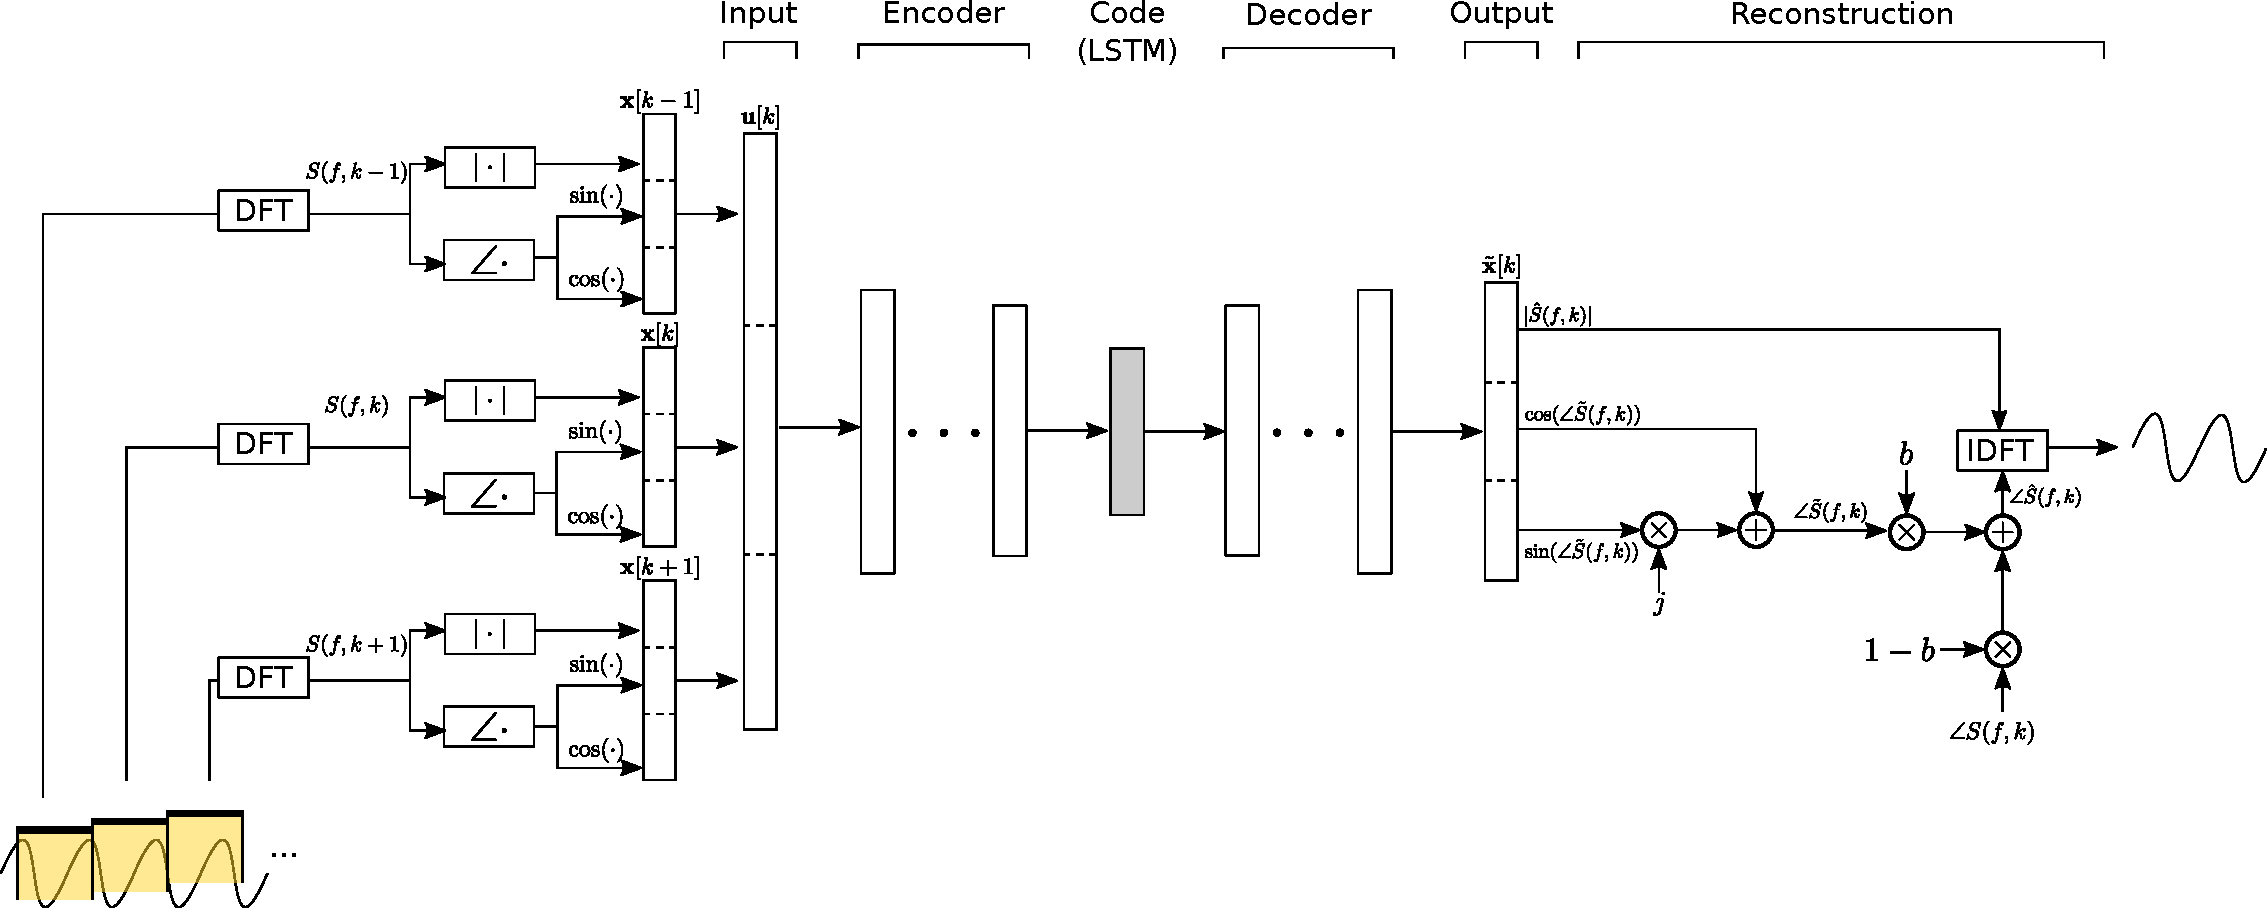
\includegraphics[width=\textwidth]{img/audioXsynth/architecture}

%	\def\svgwidth{\textwidth}
%	\input{7_other_contributions/img/audioXsynth/architecture.pdf_tex}
	\caption{Overview of the proposed architecture.}
	\label{fig:modello}
\end{figure}

Denoting with $S(f,k)$ the Short-Time Fourier Transform (STFT) at frame $k$ of an audio signal $s[n]$, the network is designed to accept an input vector $\mathbf{u}[k]$ composed of the STFT magnitude and phase of frames adjacent to the one being processed. The phase is expressed as $\sin(\phase{S(f,k)})$ and $\cos(\phase{S(f,k)})$ terms. Denoting with $\mathbf{x}[k]$ the vector
\begin{equation}
\mathbf{x}[k] = \begin{bmatrix} \left|S(f,k)\right| \\ \cos(\phase{S(f,k)}) \\ \sin(\phase{S(f,k)})  \end{bmatrix},
\end{equation} 
the network input vector $\mathbf{u}[k]$ is given by:
% \begin{equation}
%\mathbf{u}[k] =   \begin{bmatrix} \mathbf{x}[k-K] \\ \vdots \\ \mathbf{x}[k-1] \\  \mathbf{x}[k] \\ \mathbf{x}[k+1] \\ \vdots \\\mathbf{x}[k+K] \end{bmatrix}.
%\end{equation}
\begin{equation}
\mathbf{u}[k] =   \begin{bmatrix} \mathbf{x}[k-1] \\  \mathbf{x}[k] \\ \mathbf{x}[k+1] \end{bmatrix}.
\end{equation}
Indicating with $F$ the size of the FFT, the vectors $\mathbf{x}[k]$  and $\mathbf{u}[k]$ are respectively composed of $3F$ and $9F$ elements. 

The encoding section of the network is composed of a stack of fully connected layers of gradually narrower size, reaching the inner hidden layer that yields the latent code of representation. Similarly, the decoding section is composed of a stack of fully connected layers, excepts for the fact that the layer size gradually grows from the inner hidden layer to the output layer. 

The output layer of the network is composed of 3 groups of $F$ neurons, so that the output vector is arranged as $\mathbf{x}[k]$. Each group is specialized to reconstruct a component of the complex $S(f,k)$ as:
\begin{equation}
\tilde{\mathbf{x}}[k] = \begin{bmatrix} \left|\tilde{S}(f,n)\right| \\ \cos(\phase{\tilde{S}(f,k)}) \\ \sin(\phase{\tilde{S}(f,k)})  \end{bmatrix}.
\end{equation} 
The ReLU activation function is only applied to the group related to the magnitude reconstruction, in order to constrain the output values to be positive. The $\tanh$ activation function is applied to all other neurons in the architecture, in order to allow the signals to assume values in the range $[-1, 1]$.

Such a simple configuration is able to learn and reproduce an averaged spectrum, so that a dataset containing chromatic scales reproduces a signal that contains all musical notes at the same time. This is not sufficient in the current context, thus, temporal dependencies must be learned by the network.
This can be obtained by using one or more recurrent layers as inner layer of the network. In particular, we used one hidden layer composed of Long-Short Term Memory block (LSTM). These blocks can efficiently exploit a long-range temporal context by means of connections between units which form directed cycles, and store state information in the cell.


A feature-wise batch normalization is applied to the output of each layer of the network in order to  reduce the internal covariance shift and to better distribute the latent representations obtained during the network training procedure. In addition, the dropout technique was employed during the neural network training to prevent overfitting and increase the generalization performance of the neural network in reconstructing the input signal. 

Training is performed by using a dataset composed of audio signals characterized by the desired timbre. The network is trained to minimise the mean squared error between the estimated signal $\tilde{\mathbf{x}}[k]$ and the input signal $\mathbf{x}[k]$ by using the AdaDelta stochastic gradient-based optimization algorithm. It was chosen because it is well-suited for dealing with sparse data and is robust to different choices of model hyperparameters. Furthermore no manual tuning of learning rate is required.


\subsubsection{Resynthesis}
During the generation phase, a novel input is employed featuring a different instrument/timbre from the ones used during training. Special care must be taken in the inverse STFT processing in order to provide time-domain reconstruction without phase artefacts. Owing from works in cross-synthesis and spectral morphing \cite{Cella2013advanced}, the predicted spectral magnitude and phase can be mixed with the magnitude and phase of the input signal. Denoting with $\hat{S}$ the DFT of the final reconstructed signal, the output magnitude and phase are obtained as:
\begin{align}
|\hat{S}| &= a |S| + (1-a) |\tilde{S}| + a_M \sqrt{|S|\cdot|\tilde{S}|}, \label{eq:hybridmag}\\
\angle \hat{S} &= b \angle \tilde{S} + (1-b) \angle S,\label{eq:hibrydph}
\end{align}
where $0 < a,b, a_M < 1$ determine the proportion between the estimated and original signal components. In practice, the original magnitude information is not used, i.e., $|\hat{S}| =  |\tilde{S}|$, while choosing $b$ close to 0.5 allows to obtain a time domain signal with reduced artefacts. This is the choice followed for all reported experiments.

\subsection{Comparative Methods}
\label{sec:comparative}

To provide a comparison to the proposed approach, the following methods for timbre transfer have been implemented to be tested with the same audio material. The implemented algorithms are:

\begin{itemize}
	% non la abbiamo usata alla fine!!	\item \textbf{DFT morphing}: the timbre transfer is here implemented by interpolating in the parameter space of the DFT using the formulas given in equations \ref{eq:hybridmag} and \ref{eq:hibrydph} (often known as generalized cross-synthesis);
	\item \textbf{spectral envelope hybridization}: in this case, the timbre transfer is performed by computing  the spectral envelope of both signals, flattening the envelope of the target signal by deconvolution and then multiplying it by the source signal; in this context, the spectral envelope is based on the cepstrum as follows: 
	
	\begin{equation}
	E = DFT (W_{LP} (DFT^{-1} (log (|DFT (s)|))))
	\end{equation}
	where $W_{LP}$ is a low-pass filter in the cepstral domain called \textit{liftering} filter and $S$ is a signal in time domain;
	\item \textbf{MFCC-based mosaicing}: this method performs timbre transferring by replacing the frames of the source signal by specific frames of a target dataset of sounds (that we call dictionary), where the match is done by some distance measure in a specific domain; in this context, we used a \emph{k}-nn algorithm applied on the first 14 Mel-frequency cepstral coefficients (MFCC) of each frame \cite{Burred2014framework}.
\end{itemize}

For the MFCC-based approach, the length of the generated output sound is equal to the length of the input sound. For the other methods, instead, the generated output is as long as the longest between input and target, where the shorter one is repeated as necessary during the process. 

The spectral envelope hybridization and the MFCC-based mosaicing methods do not require parameters and perform a full timbre transfer between the processed signals; on the other hand, the DFT morphing requires the setting of the interpolation parameters. In this context we decided to create the output sound by using the phases of the source signal and the amplitudes of both signals while keeping some bias on the target signal. To achieve this, we set the interpolation parameters as follows: $a = 0, b = 1, a_{M} = 1$.

\subsection{Experiments}\label{sec:experiments_audiox}
\subsubsection{Experimental Setup}
The algorithm has been implemented in the Python programming language using the Keras deep learning libraries. All the experiments were performed on a CINECA Galileo computational node with Nvidia K80 accelerators.

The neural networks were trained with the Adadelta gradient descent algorithm and a learning rate equal to 1.0, $\rho=0.95$, $\epsilon=10^{-6}$. The maximum number of epochs was set to 300 and an early stopping strategy on the validation set loss with 20 epochs of patience was employed for regularization. Each training iteration involved a number of samples (i.e., batch size) between the 5\% and the 10\% of total samples present in the training set, depending on the amount of samples present on the latter. 

The network weights were initialized with a random Gaussian distribution with mean $\mu=0$ and standard deviation $\sigma=0.1$, as it usually provides an acceptable initialization in our experience. Several network topologies were tested, varying the number of layers and units per layer.
Indeed the number of layers of the encoder has been varied from 1 to 4 while the number of unit for each layer from 80 to 4096. The decoder part was mirrored with respect to the encoder. The number of LSTM layers has been varied from  0 (no LSTM layer) to 1 with a number of units from 80 to 1024.
%ranging as reporting in \ref{tab:arch_dim}.

% from 80 (Encoder), 80 (LSTM), 80 (Decoder) to 4096-4096 (E), 1024 (LSTM), 4096-4096 (D).

Two datasets have been employed for the evaluation of the proposed approach. Dataset 1 is an internal dataset of recorded solo instrumental or vocal tracks. Each audio file consisted of 30-120 seconds of audio. The following instruments were considered: clean electric guitar (2 files), distorted electric guitar (3 files), synth pad (2 file), trumpet (3 files), electric piano (3 files), male voice (1 file), female voice (2 files). All the files are real recordings of solo performance and thus contains a rich content of notes, chords (for polyphonic instruments), legatos, glissandi, and other expressive effects. Each file is played on a single tonality.

Dataset 2 is built from a very large musical instrument dataset shared by the Magenta project team\footnote{https://magenta.tensorflow.org/nsynth}, containing single notes for eleven classes of musical instruments. In creating Dataset 2 we picked ten from the eleven classes, discarding the bass class because of its narrow coverage of the frequency spectrum, and randomly selected 3500 audio files for each class, to give each class the same dimensionality. This dataset is composed of short files containing a single note each, at different dynamic levels and pitches. The differences between the two datasets have been exploited to observe the role of the training data on the resulting output.

All files from Dataset 1 have been sub-sampled to 22050\,Hz to reduce the computational cost, while the files from Dataset 2 are sampled at 16~kHz and were left as such. The STFT of the audio signals were computed with a 2048-points DFT, 50\% overlap and window size calculated in order to reach 43 frames per second.

Audio samples are available at \texttt{https://gitlab.com/a3labPapers/\\CompanionFiles/tree/master/AES-XSynth}.

\subsection{Results}
\label{sec:results}
This section reports experiments with different audio sources as target and input conducted on Dataset 1 and 2 together with a qualitative analysis of the synthesized outputs.
A first batch of experiments was conducted with Dataset 1 to tune the network hyperparameters. The outputs produced by autoencoders trained on each file in the dataset have been evaluated by analysis of their spectrograms and informal listening tests. The hyperparameters reported in Table \ref{tab:sweetparams} have been found to obtain acceptable results, which will be discussed shortly. Without considering the output layer and input layers, the network is composed of five layers: 2 layers respectively of 1024 and 808 units, one LSTM layer composed of 808 units, and 2 layers respectively of 808 and 1024 units. 

\begin{table}[t]
	\renewcommand{\arraystretch}{1.0}
	\caption{Hyperparameters used for the experiment with training on the distorted guitar track of the song \textit{Sweet Child O' Mine}.}
	\label{tab:sweetparams}
	\centering
	\begin{tabular}{c|c}
		\hline
		\textbf{Network}  \rule{0pt}{8pt} &  \multirow{2}{*}{\textbf{Dropout}} \\
		\textbf{layout}	  & \\
		\hline
		Encoder: 1024, 808  \rule{0pt}{8pt} &  input units \\
		LSTM: 808 &  to drop \\
		Decoder: 808, 1024 &   $p=0.1$ \\ 
		\hline
		\textbf{Training }  \rule{0pt}{8pt}  & \textbf{Optimiser} \\ 
		\textbf{epochs}	& 	 \textbf{parameters}\\ 
		\hline
		300, 20 patience  \rule{0pt}{8pt} & learning rate = 1 \\
		Validation split = 10\% &  $\rho=0.95$, $\epsilon=10^{-6}$ \\
		\hline
		\multicolumn{2}{c}{\textbf{Batch Normalization:}  $\epsilon = 10^{-6}$, $\mu=0.9$}  \rule{0pt}{8pt} \\
		\hline
	\end{tabular}
\end{table}

\subsubsection{Reconstruction Tests}

Preliminary tests were conducted to ensure that the autoencoder is able to reconstruct an input signal if it is also used for training. The network is able to reconstruct sufficiently well the original file, although some compression is inherent to the compressive autoencoding process. Figure \ref{fig:same} shows the spectrogram of an electric guitar from Dataset 1 playing arpeggios and chords and its reconstruction. The compression is visible from the spectrograms especially at high frequency.

\begin{figure}[t]
	\centering
	\begin{subfigure}[b]{0.5\textwidth}
		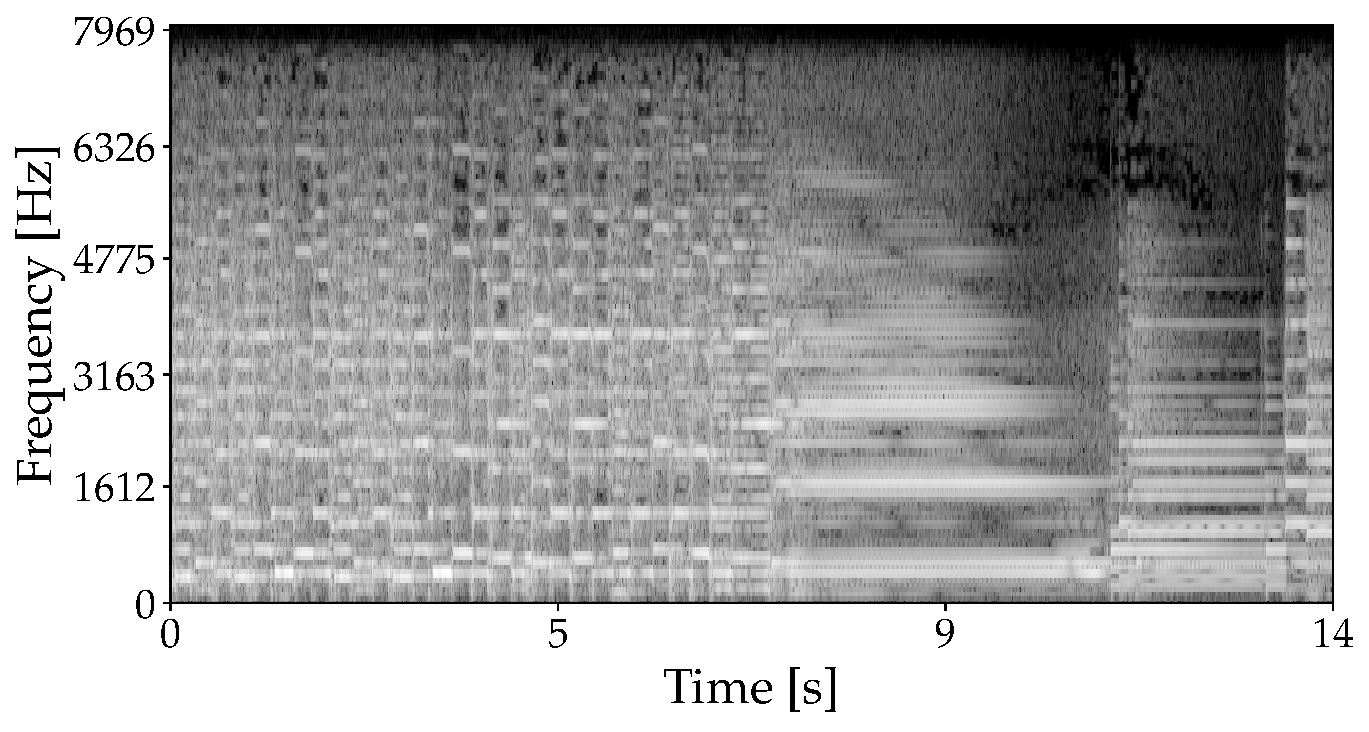
\includegraphics[width=\textwidth]{img/audioXsynth/plots/specgram_orig-Child}
		\subcaption{Original electric guitar track (input and target).}
	\end{subfigure}
	\hfil
	\begin{subfigure}[b]{0.5\textwidth}
		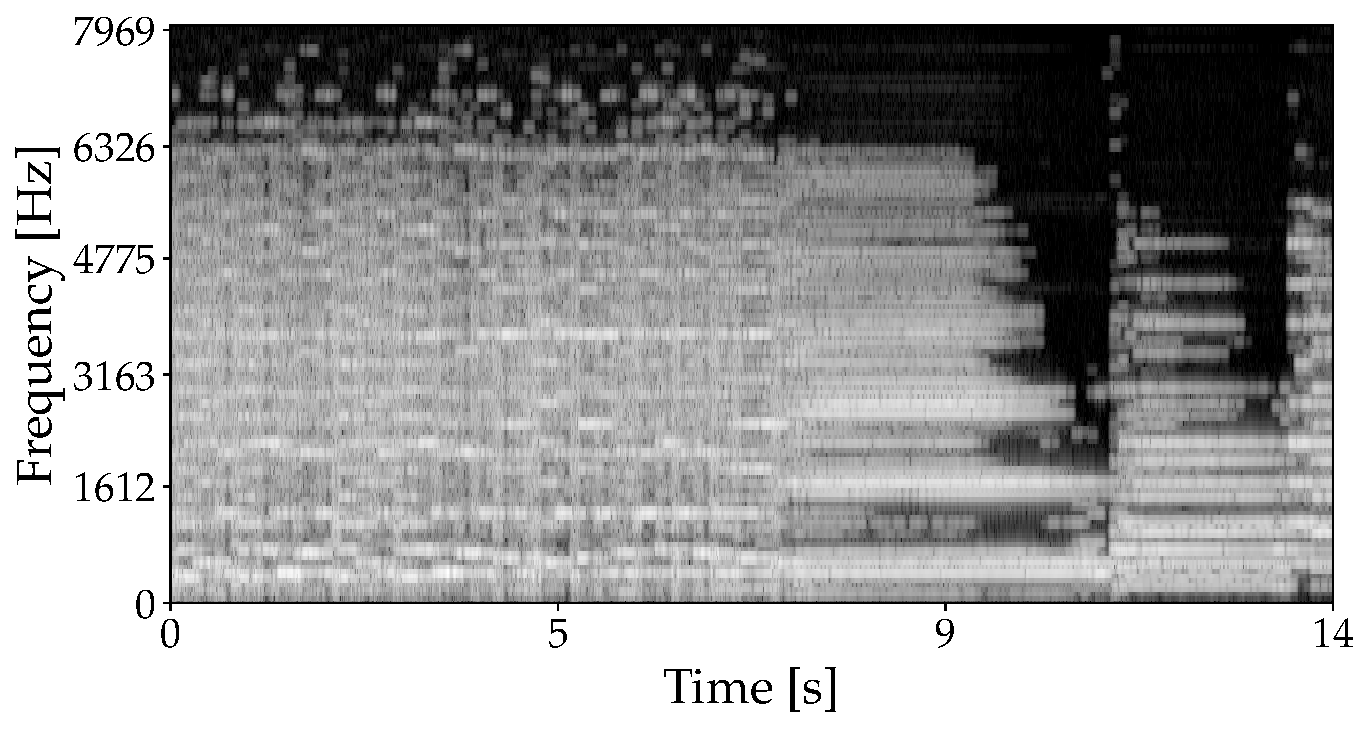
\includegraphics[width=\textwidth]{img/audioXsynth/plots/specgram_selfcodingChild}
		\subcaption{Reconstruction.}
	\end{subfigure}
	
	
	\caption{Spectrograms from (a) an electric guitar track, (b) its reconstruction when using (a) as both target and input. The hyperparameters for (b) are reported in Table \ref{tab:sweetparams}.}
	\label{fig:same}
\end{figure}

\subsubsection{Dataset 1}

These experiments were done with a female singing voice input file (from now on, in short FV1). This choice is motivated by the fact that the voice has subtle pitch variations (vibratos, glissandi, etc.) and the voice presents pitched, unpitched and unvoiced audio. 

As an example of the results that can be obtained by the proposed architecture, some selected outputs are analysed in detail. A distorted guitar track from Dataset 1 (playing the tune in \textit{Sweet Child O' Mine} by Guns N'Roses) is taken as the target for the proposed architecture with parameters shown in Table \ref{tab:sweetparams}. The resulting output file is named R1 for short, and its spectrogram is shown in Figure \ref{fig:specgrams-1}(b). For comparison, the distorted guitar track has also been used for the MFCC-based mosaicing algorithm and for the spectral flattening algorithm. The input file used for all techniques is FV1. Its spectrogram is shown in Figure \ref{fig:specgrams-1}(a), followed by the spectrograms obtained by the other methods.
%Another example is provided in Figure \ref{fig:specgrams-2} where a recording of a female singer with a distinctive breathy timbre (from now on, FV2) is used as a target and FV1 as input. The proposed approach is the only method to obtain a plausible timbre transfer from the input voice to the target voice and retains the pitch of the input file, although not all phonemes are recognizable. 

With the proposed approach, timbre is quite coherent from frame to frame if compared, for example, to the MFCC-based method, thus resulting in a more convincing output. In the MFCC hybridization, furthermore, it is also quite apparent that frames from the target signal appear from time to time in an inconsistent way exposing explicit features of the target (for example, a recognizable note in a riff). Finally, the spectral flattening method has a recognizable vocoder-like timbre, with the musical structure of the target file appearing together with its spectral content, which is an undesired feature in this context (see, for example, the arpeggios of the target song appearing in the spectrogram and chromagram approximately at 5\,s on to the end).

Chromagrams from audio files shown in Figure \ref{fig:specgrams-1} are shown in Figure \ref{fig:chromas}, to compare the pitch trajectories and the presence of spurious chromatic components. The chromagrams obtained from the proposed architecture (Figure \ref{fig:chromas}(b),(e)) show similar pitch trajectories to the input signal (Figure \ref{fig:chromas}(a)). We observe that the network fails to follow the pitch of the input when it is outside the range learned during the training phase. This can be seen around second 2 in Figure \ref{fig:chromas}(e), where the high pitch of the input file reaches a B4 which the network cannot match, due to the lack of notes above G\#4 in the training set.


\subsubsection{Dataset 2}

The experiments with Dataset 2 were conducted by training an autoencoder for each of the ten instrument classes, thus greatly increasing the complexity of the problem. Each trained autoencoder was subsequently used to synthesize audio with FV1 as input, resulting in ten audio files of different timbre and similar pitch contour. As an example of the good pitch tracking capabilities of the proposed architecture, we report a DFT (4096 points) calculated for each file at a specific time interval, where the input file shows a pitched \textit{/i:/} phoneme at frequency 497.6\,Hz (B4 + 13~cents), see Figure \ref{fig:all-dft-pos2}. Each DFT has different features (e.g., spectral slope, spectral centroid, presence of noise, etc.) but all have same pitch. 

From the experiments with Dataset 2 we observed that the network cannot follow glissando, pitch bending and vibrato from the input because the dataset has no time-varying pitch to be learned, being composed of static single notes only. This is apparent by applying FV1 as input and results in lower-quality note transitions compared to the autoencoder trained on Dataset 1. 

Judging timbre learning and transferring with this dataset is difficult because of the extremely large variety of tones in an instrument class and the large number of files to evaluate. The network cannot learn all the timbres of the different instruments in a class, but it learns instead an averaged spectrum of the whole class. It must be noted that we are not conducting supervised training in this work, thus, the network was not instructed with labels regarding the instrument type or any other property of the target sound that could help in clustering the timbre families inside a class.
The bandwidth of the output is related to that of the class used for training with, e.g.,brass instruments having a wide spectrum and flutes having a reduced bandwidth when producing an output with the same input. We also noted that the autoencoder trained on vocal samples produces tones with a voice-like texture. 


\subsubsection{Pitch Tracking Accuracy}
We conducted more systematic tests to quantify the pitch tracking accuracy of the architecture. These tests were conducted with Dataset 2 because of the precise pitch of its content and its stability over time, allowing for an easier pitch accuracy evaluation. Five audio files were generated systematically from a MIDI file containing 20 random notes. Each audio file was generated from a different digital instruments using sampling synthesis and employing equal temperament and 440.0 Hz tuning. Using the 5 files as input to the 10 networks, resulted in 50 outputs for a total of 1000 notes. 

Pitch accuracy was evaluated by employing a peak picking algorithm in the frequency domain \cite{JOSbook2_SASP}, using a thresholded parabolically-interpolated STFT\footnote{https://librosa.github.io/librosa/generated/librosa.core.piptrack.html}. %, with a STFT window size equal to 8192 points, 512 points of hop size and threshold equal to 0.9. %The conversion from pitch to note classes was done with Librosa::hz\_to\_note() function. 
For each note, the accuracy was evaluated considering 128 pitch classes (those defined by the MIDI protocol), plus one unpitched class (i.e.,the output shows no clear pitch information, despite the input content which was always pitched). A pitch tolerance of $\pm 50$ cents and an octave tolerance of $\pm 1$ were allowed.

Only 12\% of the 1000 notes lost the original pitch, showing a good reliability of the network in retaining the original pitch of the input.

\begin{figure}[t]
	\centering
	\begin{subfigure}[b]{0.48\textwidth}
		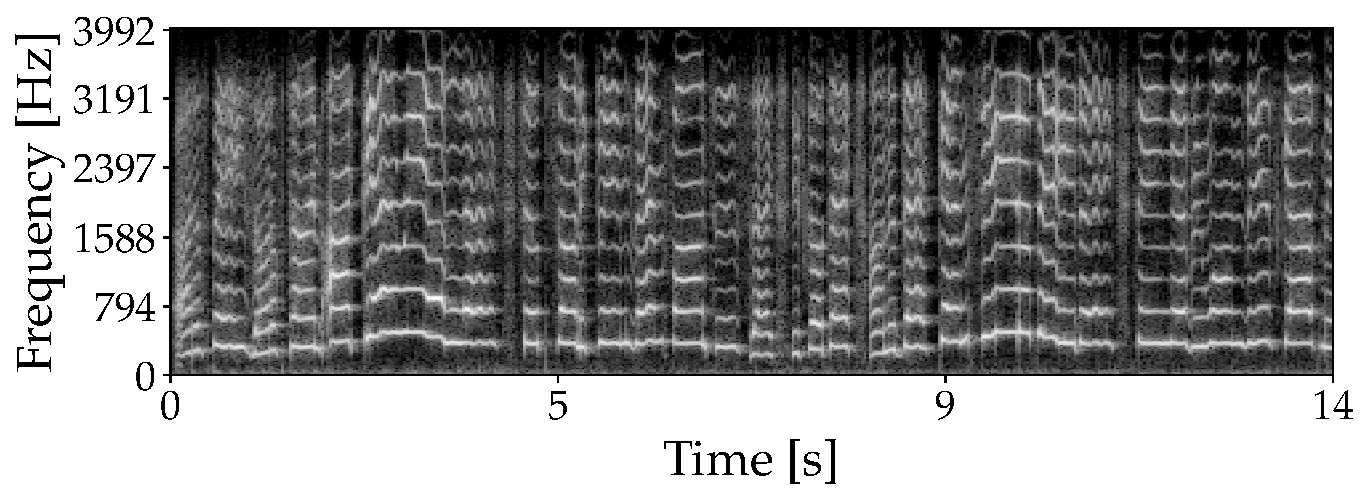
\includegraphics[width=\textwidth]{img/audioXsynth/plots/specgram_Vox}
		\subcaption{Female voice FV1 (input).}
	\end{subfigure}
	\hfil
	\begin{subfigure}[b]{0.48\textwidth}
		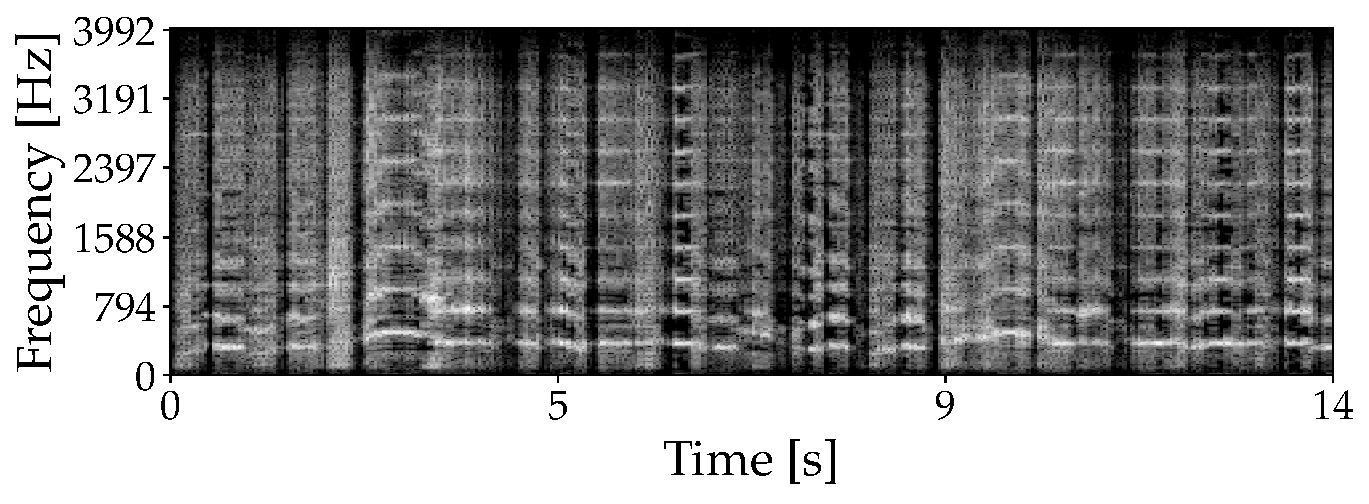
\includegraphics[width=\textwidth]{img/audioXsynth/plots/specgram_406_P_ENV}
		\subcaption{The proposed approach.}
	\end{subfigure}
	\hfil
	\begin{subfigure}[b]{0.48\textwidth}
		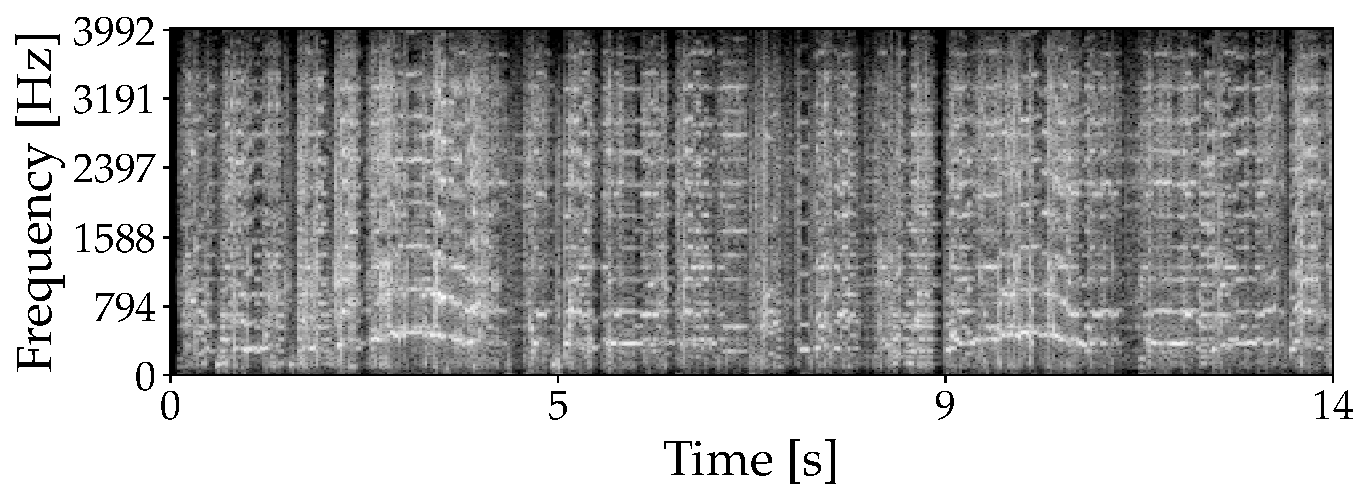
\includegraphics[width=\textwidth]{img/audioXsynth/plots/specgram_mfcc-knn}
		\subcaption{$k$-nn matching techinque.}
	\end{subfigure}
	\hfil
	\begin{subfigure}[b]{0.48\textwidth}
		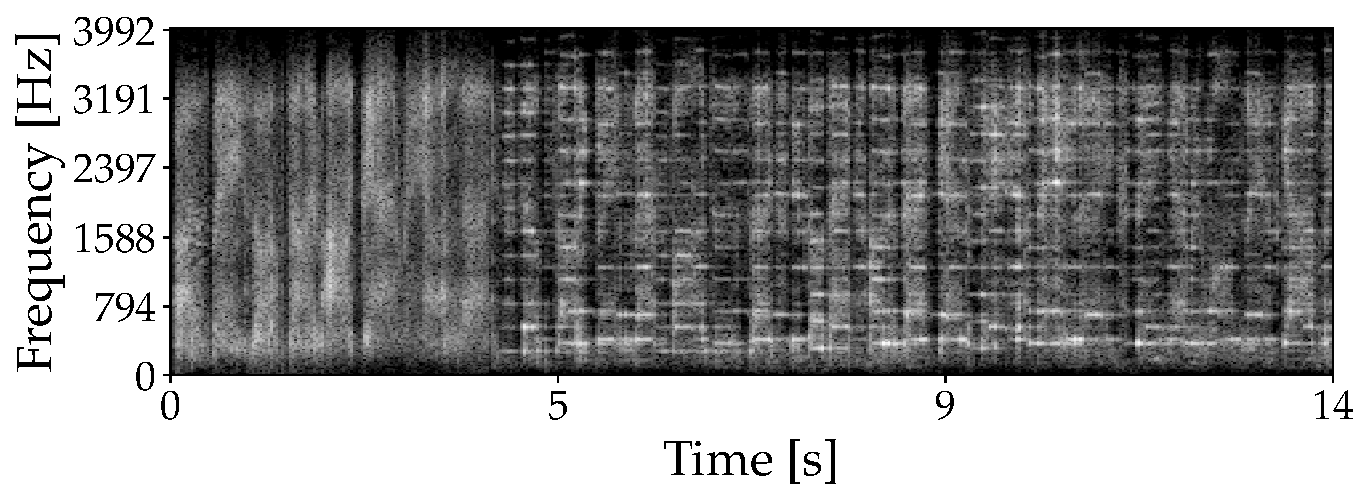
\includegraphics[width=\textwidth]{img/audioXsynth/plots/specgram_flatten}
		\subcaption{Spectral flattening technique.}
	\end{subfigure}
	
	\caption{Spectrograms from the input female voice FV1 (a), the proposed approach and the comparative methods(c-d). The hyperparameters for (b) are reported in Table \ref{tab:sweetparams}.}
	\label{fig:specgrams-1}
\end{figure}


\begin{figure}[t]
	\centering
	
	
	\begin{subfigure}[b]{0.46\textwidth}
		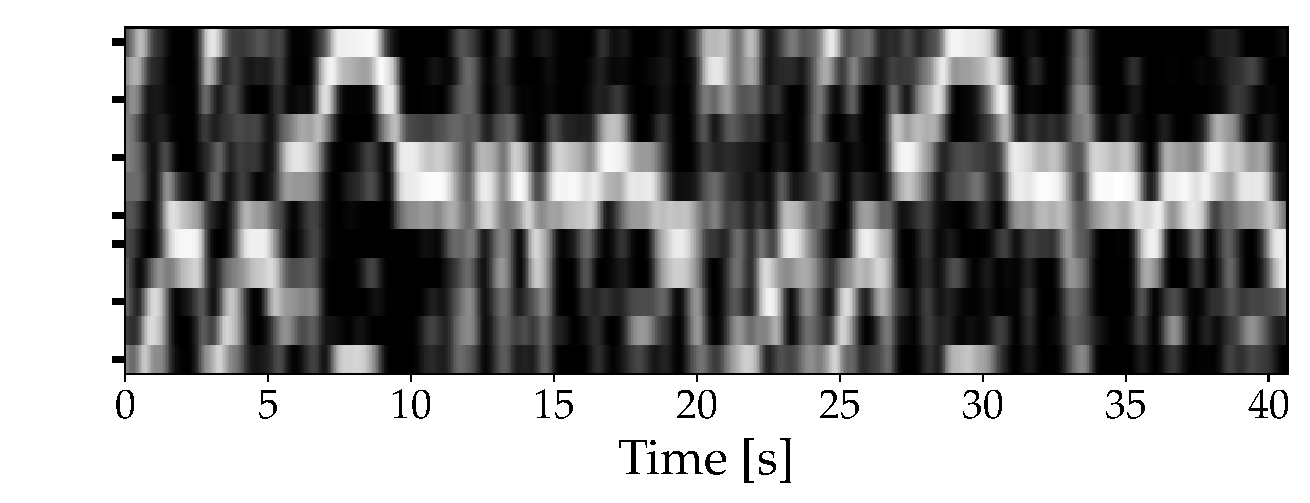
\includegraphics[width=\textwidth]{img/audioXsynth/plots/chromagram-specgram_Vox}
		\subcaption{Female voice FV1 (input).}
	\end{subfigure}
	\hfil
	
	\begin{subfigure}[b]{0.46\textwidth}
		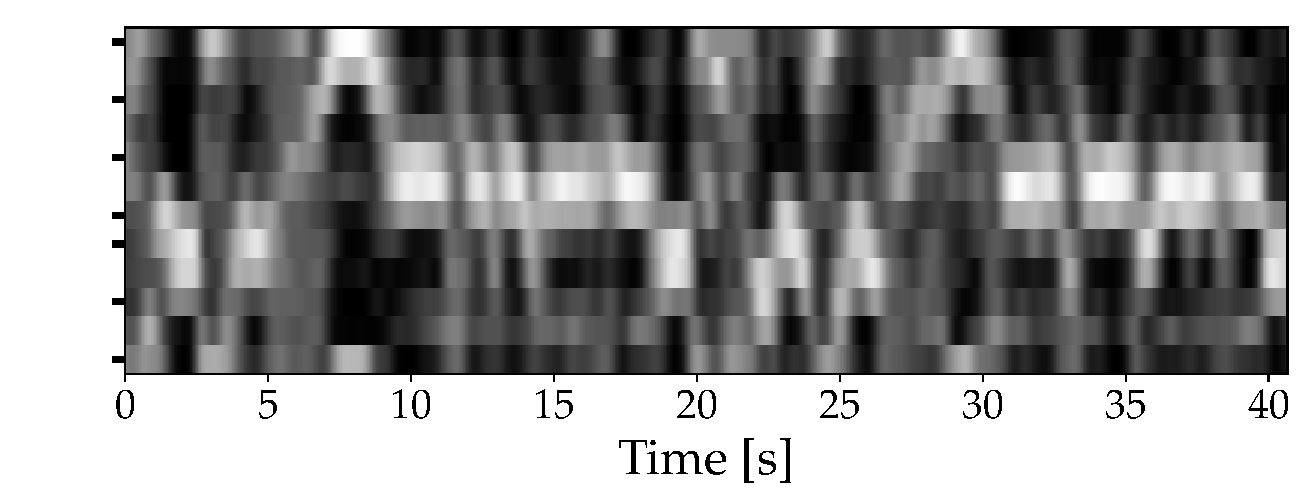
\includegraphics[width=\textwidth]{img/audioXsynth/plots/chromagram-specgram_406_P_ENV}
		\subcaption{The proposed approach.}
	\end{subfigure}
	\hfil
	\begin{subfigure}[b]{0.46\textwidth}
		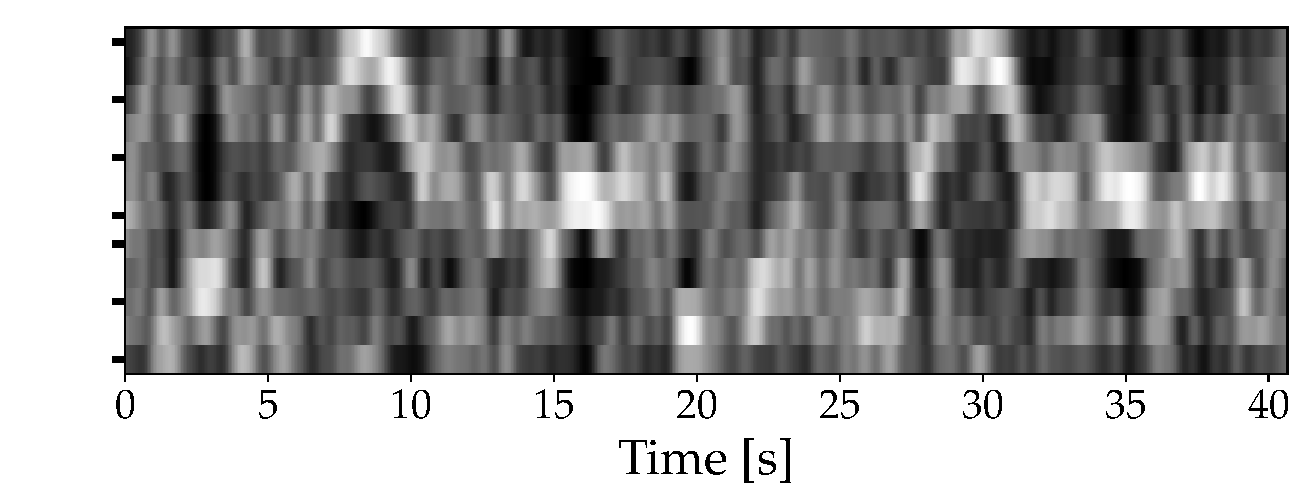
\includegraphics[width=\textwidth]{img/audioXsynth/plots/chromagram-specgram_mfcc-knn}
		\subcaption{k-nn matching technique.}
	\end{subfigure}
	\hfil
	\begin{subfigure}[b]{0.46\textwidth}
		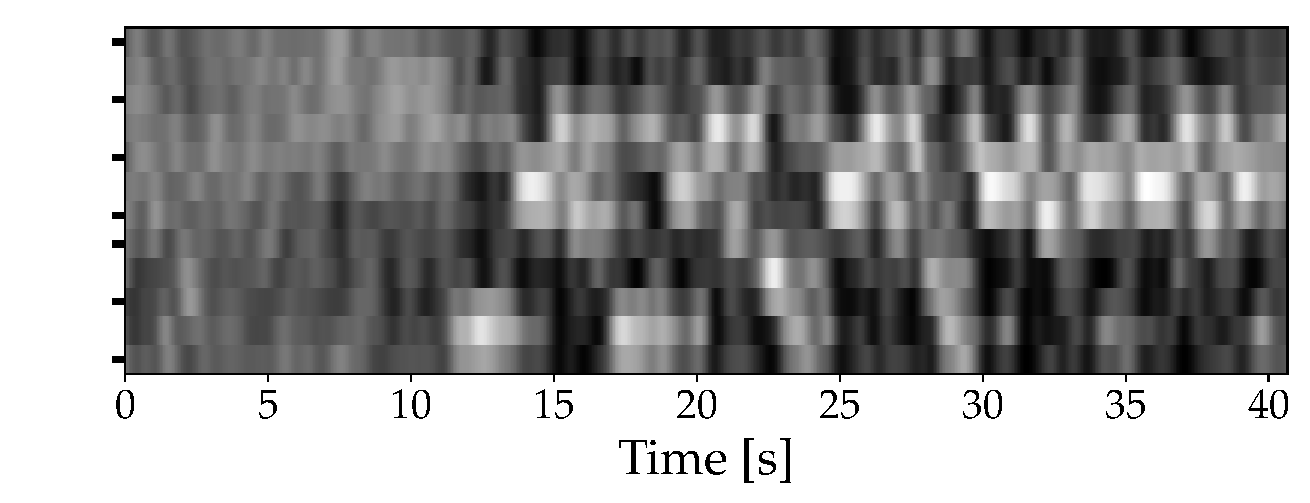
\includegraphics[width=\textwidth]{img/audioXsynth/plots/chromagram-specgram_flatten}
		\subcaption{Spectral flattening technique.}
	\end{subfigure}
	
	
	\caption{Chromagrams from (a) FV1, (b) to (d) different timbre transfer approaches using a distorted guitar track as a target and FV1 as input. Vertical axis shows the 12 notes (ticks correspond to natural notes).}
	\label{fig:chromas}
\end{figure}

\begin{figure}
	\centering
	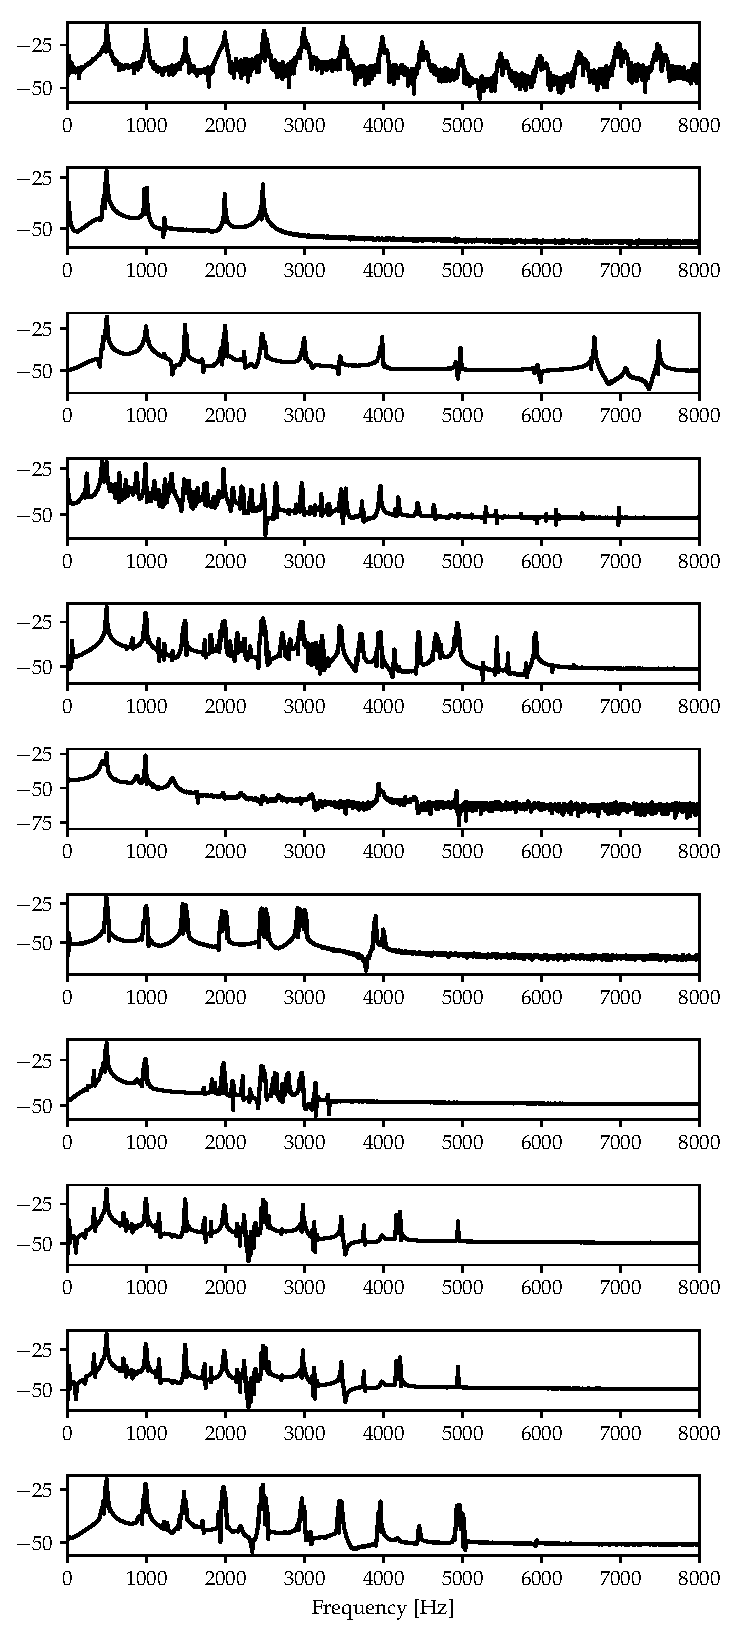
\includegraphics[width=0.8\linewidth]{img/audioXsynth/plots/vox_to_magenta/all-dft-pos2}
	\caption{Windowed DFTs taken from each instrument class output with FV1 as input, at the position where a pitched /i:/ phoneme takes places in FV1. Each DFT shows similar pitch, although timbres differ. Instrument classes, top to bottom: brass, flute, guitar, keyboard, mallet, organ, reed, string, synth-lead, vocal.}
	\label{fig:all-dft-pos2}
\end{figure}


\subsubsection{Discussion}
Overall, some properties of the proposed method are summarized.
\begin{itemize}
	\item The output pitch follows quite closely the pitch of the input signal if the training set contains pitched audio in the same range as the input, however, the network is not able to generalize above or below the pitch range learned from the target file.
	\item For multi-pitched inputs (e.g., containing chords) the network is usually able to generalize providing a harmonization similar to the input.
	\item The timbre of the output signal resembles that of the training set, if the latter is sufficiently homogeneous (e.g., solo instrument from a track or separate notes from a specific instrument).
	\item Unpitched frames in the input audio are mapped to unpitched frames in the output if the training set contains unpitched material.
	\item Spectral continuity has intermediate quality between $k$-nn approaches and whitening approaches, i.e., frames do not change abruptly, thanks to the input context and the LSTM layer, but may still have deviations on a larger time basis. Previous experiments without context and the LSTM layer resulted in an output subject to abrupt variations from frame to frame similar to mosaicing.

	\item The algorithm does not guarantee that the frame energy of the input is transferred to the output. If the training set does contain sufficient levels of dynamic to learn there is a higher chance that energy is preserved, but it is not always guaranteed. The shortcoming of this is the generation of outlier frames when the input is silent or of low energy; this can be addressed by applying the input frame energy to the output by conventional signal processing techniques, but some constraints may be applied to allow the network learning energy preservation.

\end{itemize}

The proposed architecture is also able to perform morphing in the frequency domain, according to equations \ref{eq:hybridmag}-\ref{eq:hibrydph}.

\section{Conclusion}

This work discussed how machine learning can be applied to the synthesis of novel sounds from existing sources, i.e. how it can provide a new class of \textit{transfer} algorithms that has different properties with respect to conventional algorithms for morphing, hybridization, etc. A neural autoencoder has been proposed to the task and tested with different settings. Salient properties are the ability to transfer the timbre of a training set to an input file, while preserving its pitch. Pitch preservation has been proved to be reasonably good with systematic tests, while timbre transfer still needs improvement, especially with a large corpus of input signals.

Compared to dictionary-based algorithms, such as $k$-nn matching on MFCC, it proves to be more robust in term of frame-to-frame coherence, because of its improved generalization properties and possibly more relevant frame mapping.

Nonetheless, the timbre transferring capabilities of the algorithm are not systematically evaluated because it is very sensitive to the features of its input and target signals and an evaluation framework is missing. More research work is required to make the network robust to changes in frame energy, spectral bandwidth, time decay and pitch range of the target and input audio, in order to increase the intelligibility and the quality of the output signal. Furthermore, the network must be able to generalise for pitch ranges not learned from the target signal, and must be more expressive in order to learn different timbres in a large dataset. 

%Future works will be devoted to obtain improved results by employing established convolutional techniques. Recent trends in end-to-end convolutional neural networks may bring improved timbre learning at an acceptable computational cost \cite{Pons2017audioCNN,Lee2017samplelevelDCNN}. More research effort is needed and, arguably, quantitative evaluation of the results to this extent is required. Timbre classification, following state of the art algorithms (see, e.g., \cite{Pons2017timbre}) may be regarded as a logical choice, avoiding the arbitrary selection of metrics, distances or perceptually-motivated measures.
